%%=============================================================================
%% Methodologie
%%=============================================================================

\chapter{\IfLanguageName{dutch}{Methodologie}{Methodology}}%
\label{ch:methodologie}

De eerste fase zal gewijd worden aan het analyseren van de concrete problemen die zich mogelijks kunnen voordoen bij het behouden van de originele firewall, dit kan gaan over technische en non-technische aspecten die mogelijks de dienstverlening binnen de productie kan verstoren en de financiële schade die VPK daar mogelijk zou kunnen door oplopen. Ook zal er worden gekeken hoe het implementeren van die nieuwe firewall toepassing dit probleem zouden kunnen beheren en voorkomen. Hiervoor zal er gebruik gemaakt worden van bedrijfsinterne knowledge bases, diverse papers en studies met betrekking tot netwerkbeveiliging. Zo zal er een beter inzicht te verkrijgen zijn over de mogelijke firewall opstellingen en welke strategieën er kunnen worden toegepast voor het beschermen van het ICS met behulp van firewalltoepassingen. Ook zal er worden gekeken naar andere aspecten die mogelijks spelen bij het maken van een doordachte keuze. Dit kan gaan over de ervaringen van het huidige netwerkteam met een bepaalde vendor. Maar mogelijks over de integratie met andere netwerkcomponenten en de mogelijkheid om de firewall centraal te beheren. De geschatte duurtijd van deze fase bedraagt drie dagen die verspreid zullen zijn over drie weken.


Tijdens de tweede fase zal er een interne bevraging zijn bij systeembeheerders en netwerkprofessionals op bedrijfsniveau. Hun jarenlange ervaring omtrent netwerkbeveiliging en het optimaliseren van talloze beveiligingsmaatregelen binnen VPK kan kostbare inzichten opleveren voor het achterhalen van de huidige netwerkopstelling van het bedrijf. Deze informatie zal gebruikt kunnen worden voor het configureren van de firewall zodanig dat deze optimaal geconfigureerd is in het netwerk. Zo kunnen we de schade die een aanval zou kunnen aanrichten zo minimaal mogelijk houden en zal de aanval de dienstverlening zo weinig mogelijk verstoren. Ook kan deze informatie nuttig zijn voor de evaluatie in de vijfde fase. De geschatte duurtijd van deze fase bedraagt drie dagen die verspreid zullen zijn over drie weken.

In de derde fase verwerken we de grote hoeveelheid verzamelde data om een helder overzicht te creëren. Dit maakt het makkelijker om te beslissen of we de huidige firewall opnieuw configureren of een volledig nieuwe implementeren. Deze keuze baseren we op verschillende analyses, zoals een SWOT en RASCI analyse. Hiermee brengen we niet alleen de technische voor- en nadelen in kaart, maar kijken we ook naar welke stakeholders welke taken op zich nemen na de implementatie. Op basis van deze inzichten stellen we een concreet plan op voor eventuele aanpassingen aan de firewall en het netwerk van de productiesite. De geschatte duurtijd van deze fase bedraagt twee dagen die verspreid zullen zijn over twee weken.

In het vierde deel zal er worden toegespitst op het perfectioneren van beveiligingstoepassingen. Hierbij zal er met behulp van het plan dat is opgesteld in de derde fase de huidige firewalltoepassing geherconfigureerd worden. Als er aan de hand van de verschillende analyses blijkt dat een andere firewall dan de huidige firewall een betere 'fit' zou kunnen zijn voor de eisen en noden van VPK dan kan er worden gekozen om gebruik te maken van een compleet nieuwe firewall die ook betere bescherming zal bieden tegen aanvallen op het ICS. Ook zullen er aanpassingen kunnen worden aangebracht aan de rest van het netwerk die de firewall zou kunnen helpen bij het tegenhouden van aanvallen op de ICS. De geschatte duurtijd van deze fase bedraagt drie dagen die verspreid zullen zijn over drie weken.

De vijfde en tevens laatste fase zal bestaan uit het evalueren van de impact van de geherconfigureerde firewall en de voorgestelde aanpassingen aan het netwerk. Er zullen een reeks criteria worden opgesteld waaraan voldaan moet zijn. Deze criteria zullen er voor zorgen dat we duidelijk kunnen aantonen dat mogelijke wijzigingen die we hebben aangebracht het makkelijker maken voor de systeembeheerders om de firewall te beheren en een ze ook een duidelijker inzicht krijgen van welke zaken er juist gebeuren aan de interne kant van de firewall. Daarnaast zal worden beschreven welke specifieke maatregelen het beste kunnen worden genomen om het netwerk en de firewall van het productiebedrijf beter te beschermen tegen aanvallen op de ICS. De geschatte duur van deze fase bedraagt twee dagen, verdeeld over twee weken.  

\chapter{Onderzoek}

\label{ch:onderzoek}

\section{Analyse van de huidige opstelling}

De eerste fase van dit onderzoek richt zich voornamelijk op het verzamelen van relevante informatie die nodig is voor een weloverwogen keuze van de toekomstige firewallopstelling. Bij de implementatie van IT- of OT-toepassingen binnen een productiesite moet met een groot aantal factoren rekening worden gehouden. De hoogste prioriteit van elke productiesite blijft de continuïteit van de productie. Omdat de implementatie van een nieuwe netwerktopologie verschillende risico’s met zich meebrengt, is het cruciaal om alle mogelijke problemen en scenario’s zorgvuldig in kaart te brengen. Dit voorkomt verstoringen in het productieproces en waarborgt de continuiteit van de productie.
Een verstoring van de IT-dienstverlening binnen een productiesite heeft niet alleen impact op de IT-apparaten van gebruikers, maar ook op de OT toepassingen, zoals PLC’s, sensoren en SCADA-systemen. Deze systemen spelen een belangerijke rol in het aansturen en monitoren van industriële processen. Wanneer de IT infrastructuur faalt, kunnen deze OT systemen niet meer correct functioneren, dit heeft directe gevolgen voor de productieomgeving. Daarnaast is de werking van machines binnen een productiesite sterk afhankelijk van onderlinge communicatie tussen hen. Ze zijn geprogrammeerd om in een nauwkeurige volgorde en met optimale efficiëntie te opereren, zodat de productie soepel verloopt en de supply chain niet wordt onderbroken. Als de verbinding tussen deze machines wegvalt, ontstaan er onvoorziene stilstanden en inefficiënties die de productie ernstig kunnen vertragen of zelfs volledig stilleggen. Dit heeft niet alleen gevolgen voor de interne werking van de productiesite, maar ook voor externe partners en leveranciers. Transportbedrijven, logistieke dienstverleners en andere samenwerkingspartners ervaren hinder wanneer de supply chain verstoord raakt. De expeditieafdeling, die afhankelijk is van verschillende softwaretools en netwerksystemen zoals SAP voor het plannen en coördineren van leveringen, kan haar taken niet efficiënt uitvoeren zonder een stabiele IT omgeving. Dit leidt tot vertragingen in verzendingen, problemen met voorraadbeheer en mogelijk zelfs financiële verliezen door stilstand en gemiste levertermijnen.


\subsection{Problemen met huidige OT Firewall opstelling}
In 2021 heeft VPK de productiesite van Alizay overgenomen van papierproducent Double A. Met deze overname kreeg VPK niet alleen de productiefaciliteit in handen, maar ook het volledige IT en OT netwerk dat op deze site in gebruik was. Aangezien Double A gebruikmaakte van andere leveranciers voor netwerkapparatuur en eigen best practices hanteerde voor netwerkbeheer, verschilt de opzet van dit netwerk aanzienlijk van de standaard IT/OT-infrastructuur die VPK binnen alle andere productiesites gebruikt.
Het overgenomen netwerk heeft diverse problemen met de stabiliteit, veiligheid en efficiëntie die de IT en OT systemen in gevaar brengen. Compatibiliteitsproblemen tussen de originele infrastructuur van Alizay en de standaarden van VPK maken het lastig om systemen correct te integreren met elkaar.
 
Om te beginnen is het OT-netwerk van deze site beveiligd met een firewall van het merk Sophos. Dit vormt een uitdaging, aangezien VPK standaard gebruikmaakt van Palo Alto firewalls voor de beveiliging van alle andere productiesites die ze beheren. Palo Alto biedt een centrale webinterface, genaamd Strata Cloud Manager(SCM), waarmee alle geïmplementeerde firewalls binnen het netwerk op één platform kunnen worden beheerd.

Omdat Sophos-firewalls niet compatibel zijn met SCM, moeten ze afzonderlijk worden beheerd via een eigen online portaal. Dit leidt tot een versnipperde beheeromgeving, waarin netwerkbeheerders meerdere systemen moeten gebruiken om de verschillende firewalls te beheren. Hierdoor neemt de complexiteit toe en wordt het lastiger om een uniforme beveiligingsstrategie te hanteren.

Een bijkomend voordeel van Strata Cloud Manager is dat het niet alleen een centraal overzicht biedt van alle Palo Alto firewalls, maar ook de mogelijkheid geeft om firewallregels op één plek te beheren en automatisch uit te rollen naar specifieke firewalls binnen het netwerk. Dit maakt het eenvoudiger om wijzigingen consistent door te voeren en minimaliseert de kans op fouten bij handmatige configuraties.
Daarnaast kan het gebruik van verschillende firewallmerken leiden tot inconsistente security policies, verhoogde operationele lasten en een grotere kans op menselijke fouten bij configuraties en monitoring. Om een efficiënter en gestroomlijnder netwerkbeheer te realiseren, zou het migreren van de Sophos firewall naar een andere firewalloplossing, zoals Palo Alto, een logische volgende stap zijn.

Daarnaast heeft niemand binnen het huidige netwerkteam van VPK ervaring met het implementeren en configureren van Sophos firewalls. Hoewel dit op dit moment geen direct probleem vormt voor de huidige firewallopstelling, is het wel een belangrijke factor om in overweging te nemen. Op langere termijn kan het gebrek aan expertise leiden tot verschillende uitdagingen, zoals een incorrecte configuratie van de firewalls door onvoldoende kennis van de specifieke implementatie- en beheerprincipes van Sophos.

Een verkeerde configuratie kan resulteren in beveiligingsrisico’s, verminderde netwerkprestaties of zelfs netwerkstoringen. Om deze risico’s te beperken, kan er overwogen worden om over te stappen op een firewalloplossing die beter aansluit bij de bestaande kennis en beheertools binnen VPK zoals een firewall van Palo Alto.

\begin{figure}[H]
    \centering
    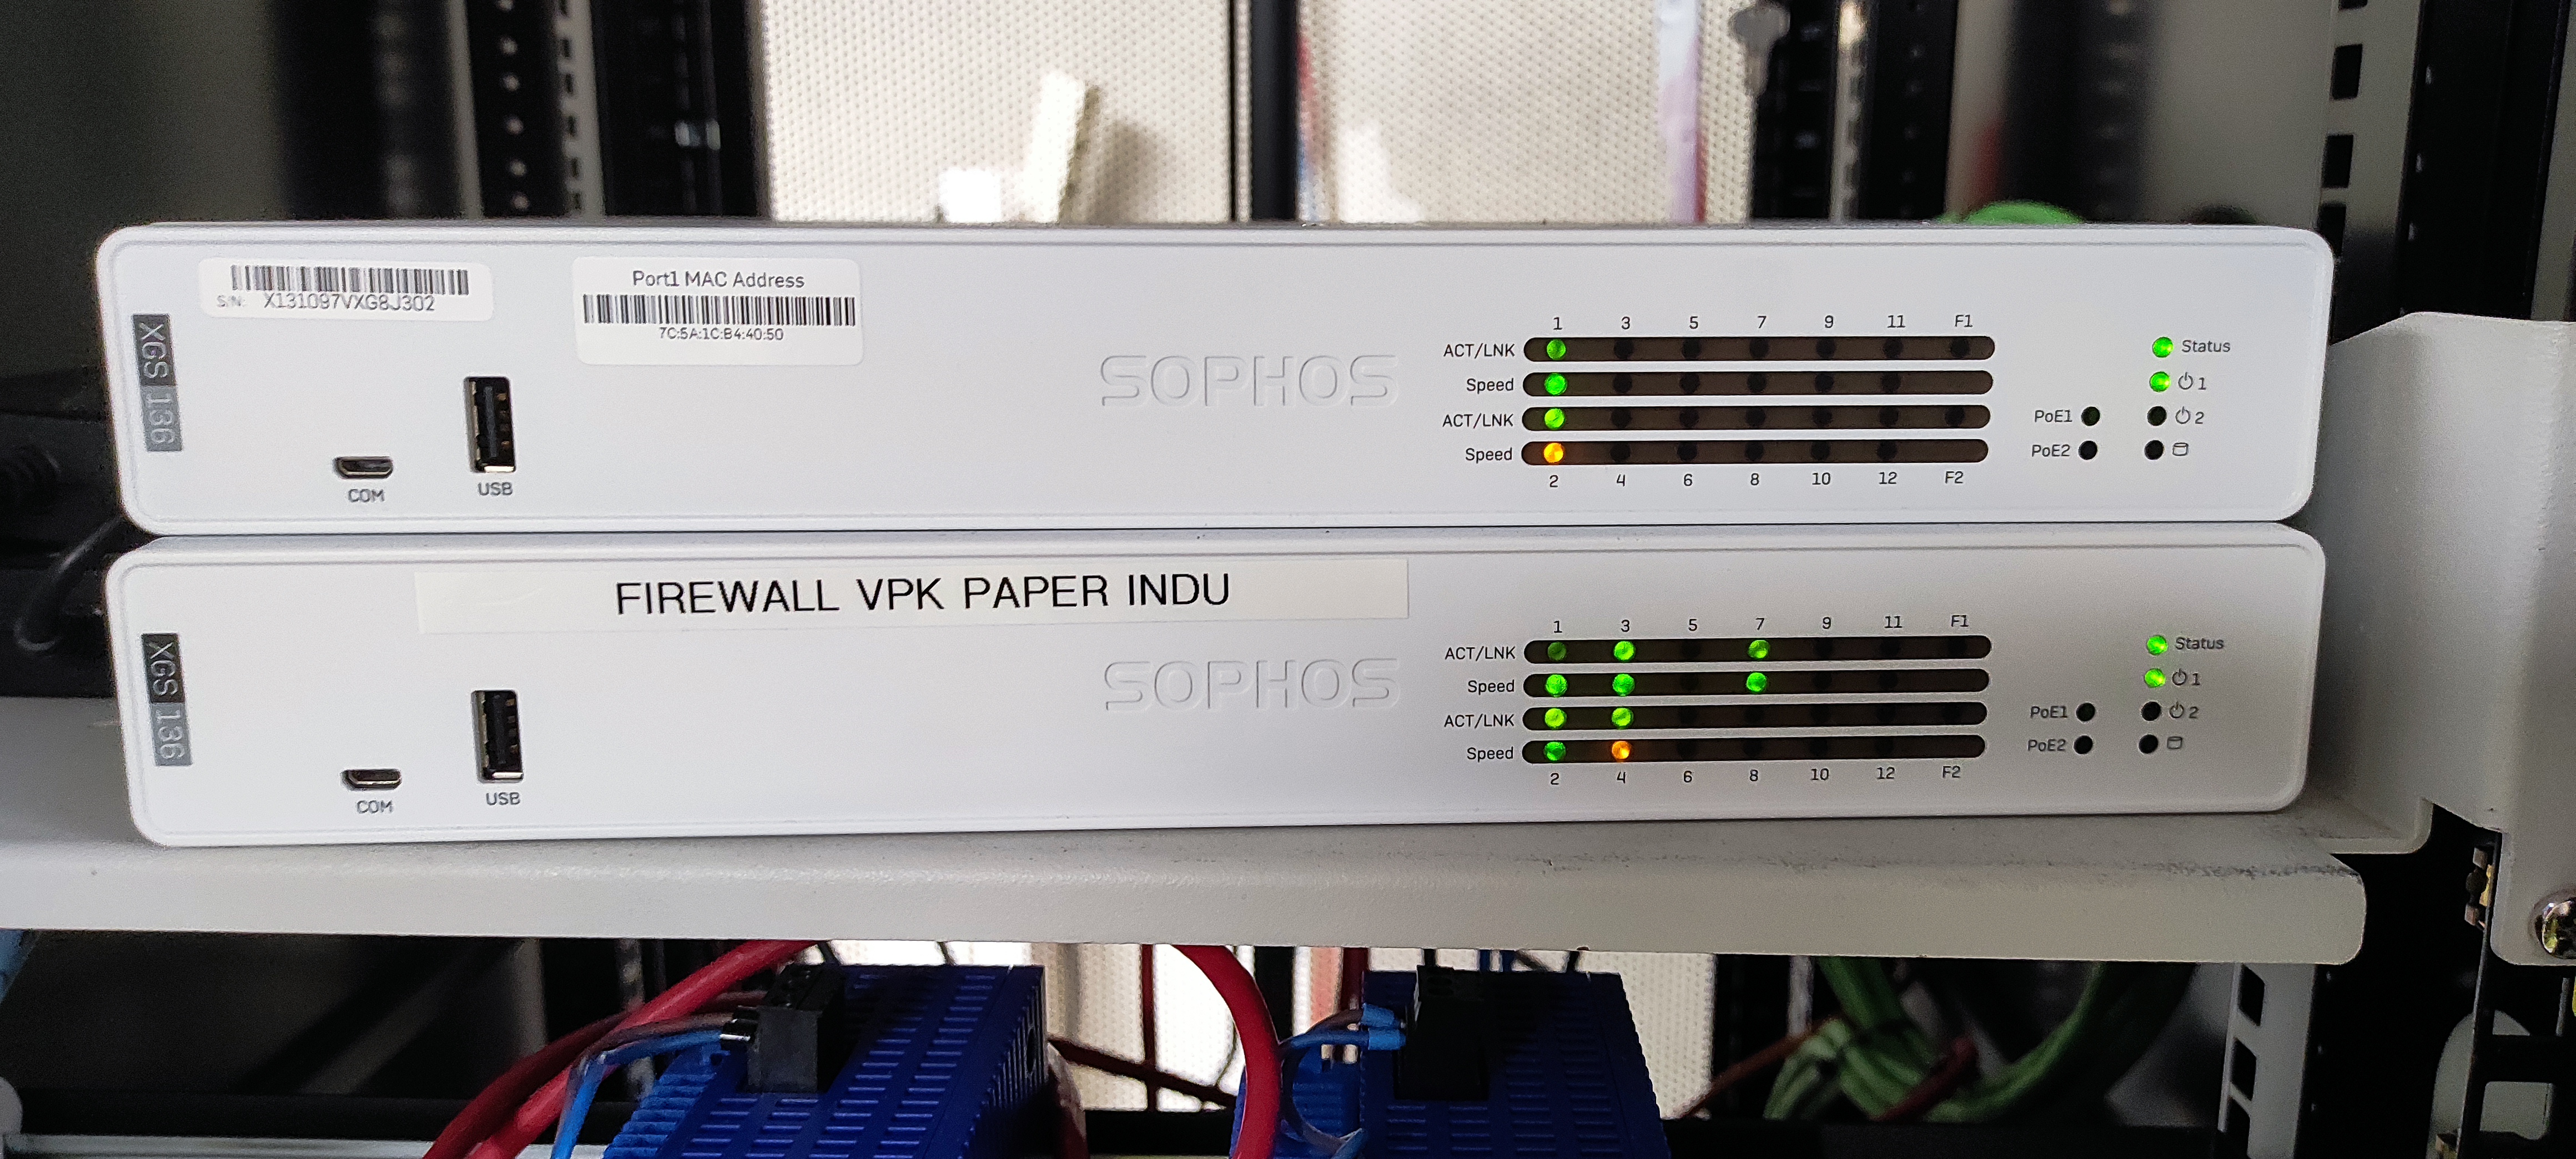
\includegraphics[width=0.8\textwidth]{fotos/SophosFirewall.jpg}
    \caption[Sophos Firewall]{\label{fig:grail}De huidige Sophos firewall die gebruikt wordt op de FR16 site van VPK.}
\end{figure} 

\subsection{Problemen met het huidige OT netwerk}
Een van de grootste uitdagingen binnen het netwerk van de productiesite van Alizay is het gebrek aan documentatie over de bestaande infrastructuur. Het netwerkteam dat verantwoordelijk was voor het onderhoud van het IT- en OT-netwerk voor de overname door VPK heeft geen gedetailleerde documentatie bijgehouden over de netwerkarchitectuur. Dit maakt het beheer van het netwerk moeilijker, omdat er onvoldoende beschikbaar is over de werking en samenstelling ervan. Zonder deze kennis wordt het uitdagend om aanpassingen door te voeren, storingen snel op te lossen en beveiligingsrisico’s effectief te beheersen.
Het OT-netwerk binnen de site van Alizay bestaat uit meerdere generaties componenten die in de loop van tientallen jaren zijn geïmplementeerd. Hierdoor is het netwerk geleidelijk uitgebreid met verschillende subnetwerken die doorheen de jaren zijn toegevoegd, vaak zonder een plan of duidelijke standaardisatie. Dit heeft geleid tot een complexe en gefragmenteerde infrastructuur, waarbij verschillende systemen en protocollen naast elkaar bestaan.
Deze gelaagde netwerkstructuur kan verschillende uitdagingen veroorzaken wanneer wordt besloten de huidige firewallregels te herzien of te optimaliseren. Op dit moment zijn er geen specifieke firewallregels die expliciet bepalen welke data uit de verschillende subnetwerken mag worden doorgelaten of geblokkeerd. Dit betekent dat het netwerk mogelijk meer verkeer toestaat dan strikt noodzakelijk is, wat een potentieel beveiligingsrisico vormt. Tegelijkertijd zorgt het ontbreken van een duidelijke segmentatie van het netwerk ervoor dat ongewenste blokkades kunnen optreden wanneer nieuwe firewallregels worden ingevoerd.
De combinatie van een verouderde netwerkinfrastructuur en het gebrek aan een goed gedefinieerd firewallbeleid kan het risico met zich mee brengen dat bepaalde subnetwerken of systemen onverwacht worden geblokkeerd bij herconfiguratie van de firewall. Dit kan ertoe leiden dat machines tijdelijk uitvallen, wat een negatieve impact heeft op de productieprocessen en de volledige supply chain. In sommige gevallen kan zelfs een kleine onderbreking in de netwerkcommunicatie ervoor zorgen dat een machine niet meer correct functioneert, waardoor productiestilstand ontstaat en de continuiteit van de productie niet gewaarborgd kan worden.

Binnen de verschillende productiesites van VPK wordt gebruikgemaakt van machines afkomstig van diverse externe leveranciers. Deze geavanceerde machines bevatten vaak een combinatie van verschillende technische componenten, zoals PLC’s, sensoren, pneumatische systemen, robotarmen en geautomatiseerde transportsystemen zoals die van Minda. 

\begin{figure}[H]
    \centering
    \includegraphics[width=0.8\textwidth]{fotos/MindaConveyorFotoBP.jpg}
    \caption[TEMP Minda]{\label{fig:grail} Een Minda conveyor installatie die pallets met kartonnen dozen verplaatst. ©Talina Scholz}
\end{figure} 

Deze componenten zijn onderling afhankelijk en wisselen continu data uit om productieprocessen op elkaar af te stemmen. Om deze gegevensuitwisseling mogelijk te maken moet er een betrouwbaar netwerk aanwezig zijn die alle verschillende componenten met elkaar verbindt.
In de praktijk betekent dit dat fabrikanten van deze machines vaak genoodzaakt zijn om hun eigen kleine netwerken op te zetten binnen de productiesite. Dit gebeurt met behulp van netwerkcomponenten zoals switches en routers, zodat hun machines correct kunnen functioneren. Wanneer een productiesite veel verschillende machines van uiteenlopende fabrikanten bevat, ontstaat al snel een situatie waarbij een groot aantal afzonderlijke private netwerken naast elkaar bestaat. Omdat deze netwerken zelden op elkaar worden afgestemd of gestandaardiseerd, leidt dit tot een uiterst gefragmenteerde netwerkstructuur. Hierdoor wordt het uniform beheren van de netwerken op verschillende VPK-sites vrijwel onmogelijk, aangezien elke site een unieke combinatie van leveranciers, machines en netwerktopologieën bevat.
Daarnaast vereisen veel fabrikanten een externe verbinding met hun machines om op afstand onderhoud te kunnen uitvoeren, real-time monitoring mogelijk te maken of software-updates te installeren. Dit betekent dat er op de productiesite van Alizay op twee mogelijke manieren een connectie met het internet kan worden gerealiseerd. De eerste optie is dat de fabrikant gebruikmaakt van het bestaande bekabelde netwerk van de site, dat wordt beheerd door VPK. In dit geval moet er bij de configuratie van de firewallregels rekening mee worden gehouden dat dit verkeer niet per ongeluk wordt geblokkeerd, anders verliest de fabrikant de mogelijkheid om zijn machines op afstand te beheren.
De tweede optie is dat de fabrikant een 4G-router met een eigen SIM-kaart gebruikt, zodat er geen directe verbinding met het netwerk van VPK nodig is. Hoewel dit in sommige gevallen een veiliger alternatief lijkt, introduceert het ook uitdagingen op het gebied van toezicht en controle over externe verbindingen. Soms kan het ook zijn dat een externe fabrikant gebruik maakt van een 4G-router en een fysieke verbinding met het VPK netwerk. In feite zal de fabrikant hierdoor de firewall gaan omzeilen. Dit is een uiterst kwetsbaar fenomeen dat veel schade kan berokken aan het VPK netwerk. Omdat in feite de firewall omzeild zal worden.
Beide methoden brengen aanzienlijke beveiligingsrisico’s met zich mee. Veel van de private netwerken die door machinefabrikanten worden opgezet, voldoen niet aan de meest recente cybersecuritystandaarden. Dit betekent dat ze kwetsbaar kunnen zijn voor aanvallen van buitenaf. Indien een hacker erin slaagt toegang te krijgen tot zo’n slecht beveiligd netwerk, kan dit een potentiële ingang vormen naar het bredere IT- en OT-netwerk van de productiesite. Dit zou ernstige gevolgen kunnen hebben, zoals productieonderbrekingen, verlies van kritieke data en zelfs de manipulatie van industriële processen.




\section{SWOT Analyse}
Een SWOT-analyse is handig om een duidelijk beeld te krijgen van een situatie. Het laat zien wat goed gaat en wat beter kan. Ook helpt het om opportunities te ontdekken en mogelijke threats op tijd te zien. Door alles op een rij te zetten, worden er geen belangrijke dingen vergeten. Dit maakt het makkelijker om goede keuzes te maken. Het helpt ook om beter na te denken over wat wel en niet werkt. Met een SWOT-analyse is er meer grip op de situatie. Dit zorgt ervoor dat de kans op succes groter wordt. SWOT staat voor Strengts, Weaknesses, Opportunities en Threats. Deze vier woorden worden hieronder verder in detail besproken.


\subsection{Strengths}
\begin{itemize}
\item \texttt{\textbf{Extra laag bescherming:} Er is al een Palo Alto (PA) firewall aanwezig, wat betekent dat de Sophos firewall een extra laag van bescherming biedt. Dit is positief omdat het netwerk al enige beveiliging heeft, en de extra firewall kan helpen om de beveiliging verder te versterken.}

\item \texttt{\textbf{De setup werkt, ook al is hij niet optimaal:} De huidige netwerkconfiguratie werkt wel, ook al is hij niet perfect. Dit betekent dat er geen grote storingen of onderbrekingen zijn, maar er is nog ruimte voor verbetering.}


\end{itemize}

\subsection{Weaknesses}

\begin{itemize}
\item \texttt{\textbf{Complexiteit door de Sophos firewall:} De Sophos firewall maakt het netwerkbeheer onnodig complex. Deze firewall voegt weinig extra waarde toe, maar maakt troubleshooting en het algemene beheer moeilijker. Het zou efficiënter zijn om een uniformere oplossing te hebben die makkelijk centraal te beheren is zoals een Palo Alto firewall.}

\item \texttt{\textbf{Problemen met switches en netwerkinfrastructuur:} Er zijn loops in het netwerk, unmanaged switches die fysiek niet bereikbaar zijn voor VPK, en oude HP switches die verouderd zijn. Deze zaken maken het netwerk moeilijker te beheren en kunnen leiden tot onverwachte storingen.}

\item \texttt{\textbf{Gebrek aan documentatie:} Het netwerk is slecht gedocumenteerd en niemand binnen het OT/IT team van Alizay kent de volledige netwerktopologie. Dit maakt het lastig om het netwerk te beheren, te troubleshooten of wijzigingen door te voeren zonder risico’s.}

\item \texttt{\textbf{Slechte firewallconfiguratie:} De huidige configuratie van de Sophos firewall is niet optimaal. Er zijn onnodige statische routes en ineffectieve firewallregels, wat zorgt voor extra complexiteit en mogelijk ook kwetsbaarheden in de beveiliging.}

\item \texttt{\textbf{Verouderde switches:} De HP switches die al sinds 2002 in gebruik zijn, hebben geen updates meer ontvangen. Dit maakt ze kwetsbaar voor beveiligingsrisico’s en zorgt ervoor dat ze niet optimaal functioneren. Ook zal hun ouderdom er voor zorgen dat er een grotere kans is op het falen van één of meerdere van hun onderdelen. Hierdoor is de kans dat er een outage is van één van deze devices een pak groter. }
\end{itemize}
    
\subsection{Opportunities}

\begin{itemize}
\item \texttt{\textbf{Uniformiteit creëren door de Sophos firewall te verwijderen:} Door de Sophos firewall te verwijderen, kan het netwerk binnen alle VPK-sites op dezelfde manier worden ingericht. Dit maakt het beheer veel eenvoudiger en efficiënter, doordat er één gestandaardiseerde opstelling is.}

\item \texttt{\textbf{Vervangen van oude switches:} De verouderde HP en hirschmann switches kunnen worden vervangen door modernere en efficiëntere modellen van Hirschmann of Cisco. Dit verbetert de prestaties van het netwerk en maakt het veiliger in het geheel.}

\item \texttt{\textbf{Netwerkinfrastructuur documenteren:} Door de huidige opstelling te wijzigen is een kans om de nieuwe netwerkstructuur goed te documenteren, wat het beheer en de troubleshooting in de toekomst veel gemakkelijker maakt.}

\item \texttt{\textbf{Vermijden van cyberdreigingen:} Door oude apparatuur en slechte configuraties te vervangen, wordt de kans op cyberaanvallen en netwerkuitval aanzienlijk verkleind. Dit verhoogt de algemene beveiliging van het netwerk.}

\item \texttt{\textbf{Segmentatie toepassen:} Er is de mogelijkheid om de netwerksegmentatie correct toe te passen, wat de beveiliging en efficiëntie van het netwerk verder kan verbeteren. Dit zorgt ervoor dat verschillende delen van het netwerk beter beschermd worden tegen dreigingen van buitenaf.}

\end{itemize}


\subsection{Threats}

\begin{itemize}
\item \texttt{\textbf{Verwijdering van de Sophos firewall kan problemen veroorzaken:} Omdat de Sophos firewall diep verweven is in het netwerk, kan het verwijderen ervan onverwachte problemen veroorzaken. Het netwerk kan niet direct goed functioneren zonder aanpassingen, wat risico’s voor de stabiliteit met zich meebrengt.}

\item \texttt{\textbf{Onbekende impact bij het verwijderen van een firewall:} Aangezien het netwerk niet goed gedocumenteerd is, kan het verwijderen van de firewall invloed hebben op onontdekte delen van het netwerk. Dit kan leiden tot onverwachte onderbrekingen of storingen.}

\item \texttt{\textbf{Externe partners kunnen beïnvloed worden:} Er zijn veel externe partners die met het netwerk verbonden zijn, zoals S2I, Evrest, en Valmet. Aanpassingen in het netwerk kunnen gevolgen hebben voor hun apparaten en systemen. Het is dus belangrijk om goed overleg te voeren met deze leveranciers om problemen te voorkomen.}

\item \texttt{\textbf{Moeilijkheden bij storing:} Als er een probleem is met netwerk apparatuur (zoals switches of routers), kan het voor het IT team van VPK heel lastig zijn om de oorzaak van het probleem snel te vinden. Dit kan leiden tot lange downtime en verstoringen in de productie.}
\end{itemize}


\section{RASCI Analyse}

Volgens \textcite{Epam2024} is RASCI een raamwerk dat specifieke rollen en verantwoordelijkheden toekent aan belanghebbenden die betrokken zijn bij een project of proces. Zie het als een routekaart die iedereen naar een gezamenlijk doel leidt zonder verwarring of vertraging. 
De verschillende letters van RASCI staan voor een bepaald woord dat een bepaalde rol samenvat.

\begin{itemize}
    \item \texttt{\textbf{Responsible:} De rol die de taak effectief uitvoert. Deze persoon of groep is de drijvende kracht achter de uitvoering van de taak. }
    \item \texttt{\textbf{Accountable:} De eindverantwoordelijke voor de taak. Deze rol draagt de verantwoordelijkheid voor het uiteindelijke succes of falen van de taak. }
    \item \texttt{\textbf{Supportive:} Een rol die ondersteuning biedt aan de 'Responsible' bij het uitvoeren van de taak. }
    \item \texttt{\textbf{Consulted:} Een persoon of rol die waardevolle input levert. Zij worden geraadpleegd voor advies en meedenken bij belangrijke beslissingen.}
    \item \texttt{\textbf{Informed:} De rol die op de hoogte wordt gehouden van beslissingen of acties die binnen de taak plaatsvinden.}
\end{itemize}

\subsection{Opbouw van de RASCI Matrix.}
Volgens \textcite{Cabanillas2011} is een RASCI-matrix is opgebouwd uit twee assen: op de horizontale as worden de verschillende rollen binnen het project weergegeven, terwijl de verticale as de diverse taken toont. In elk vakje van de matrix wordt met een enkele letter aangeduid welke rol welke verantwoordelijkheid opneemt voor een bepaalde taak. Zo staat bijvoorbeeld de letter 'R' voor "Responsible. Wanneer bijvoorbeeld de letter 'R' in een bepaald vakje voorkomt, betekent dit dat de overeenkomstige rol op de horizontale as Responsable is voor de taak op de verticale as. \autocite{Cabanillas2011}

\subsection{Verschillende taken binnen deze RASCI matrix}
\textbf{Inventarisatie van bestaand OT netwerk.}
\begin{itemize}[label=\textbullet]
    \item Deze taak omvat het in kaart brengen van alle apparaten binnen het OT-netwerk van FR16. Van elk toestel worden relevante gegevens geregistreerd, zoals het MAC-adres, IP-adres, merk, type en andere nuttige informatie.  
\end{itemize}

\textbf{Onderhouden documentatie van het OT netwerk.}
\begin{itemize}[label=\textbullet]
    \item Wanneer er wijzigingen plaatsvinden binnen het netwerk (zoals het toevoegen of verwijderen van apparaten) wordt de inventarisatie hierop aangepast. Het doel is om steeds te beschikken over een actueel netwerkplan van het OT netwerk, zodat de documentatie up-to-date blijft. 
\end{itemize}

\textbf{1st line support bieden.}
\begin{itemize}[label=\textbullet]
    \item  First-line support betreft het bieden van eerste hulp bij technische problemen of meldingen. De verantwoordelijke persoon is het eerste aanspreekpunt en probeert de meldingen zo snel en efficiënt mogelijk op te lossen, of indien nodig door te verwijzen naar een volgende ondersteuningslijn.
\end{itemize}

\textbf{Beheren van netwerkkasten externe leverancier}
\begin{itemize}[label=\textbullet]
    \item Binnen de OT-omgeving bevinden zich meerdere netwerkkasten met apparatuur van externe leveranciers, waaronder switches, routers en VPN-routers. Deze componenten zijn essentieel voor de werking van de productie-installaties. 
\end{itemize}

\textbf{Beheren van fysieke componenten binnen het OT netwerk.}
\begin{itemize}[label=\textbullet]
    \item Deze taak richt zich op het beheer van industriële hardware binnen het OT-netwerk, zoals industriële switches, PLC’s, SCADA-systemen, sensoren, en andere verbonden componenten die een directe rol spelen in de operationele processen.
\end{itemize}


\textbf{Beheren van fysieke componenten binnen het IT netwerk.}
\begin{itemize}[label=\textbullet]
    \item De fysieke componenten waar men het hier over heeft zullen voornamelijk bestaan uit: switches, routers, firewalls, servers, bekabeling, …
\end{itemize}

\textbf{Onderhouden OT firewall.}
\begin{itemize}[label=\textbullet]
    \item Binnen de huidige OT opstelling van FR16 is er een Sophos firewall aanwezig. Deze firewall wordt enkel gebruik binnen het OT netwerk. Daarom is het OT team verantwoordelijk voor het beheer van deze firewall.
\end{itemize}



\begin{figure}[H]
    \centering
    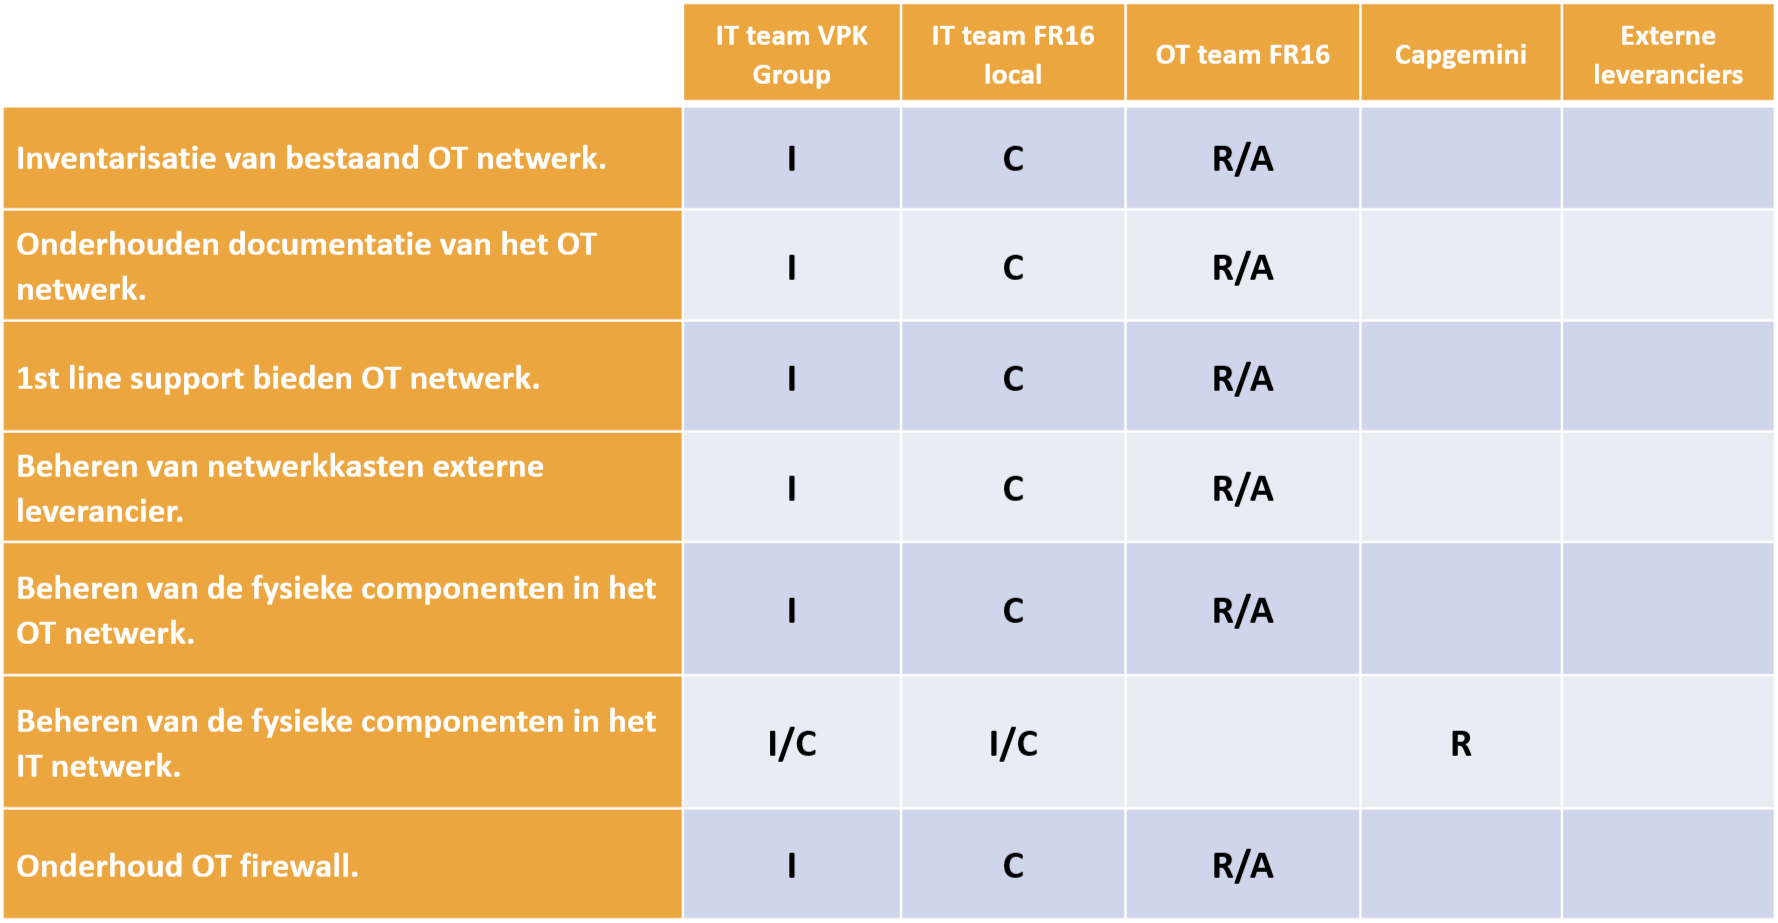
\includegraphics[width=0.9\textwidth]{fotos/Rasci_AS-IS.png}
    \caption[Foto Rasci AS-IS]{\label{fig:grail}Rasci tabel van de huidige toestand in FR16.}
\end{figure} 

\begin{figure}[H]
    \centering
    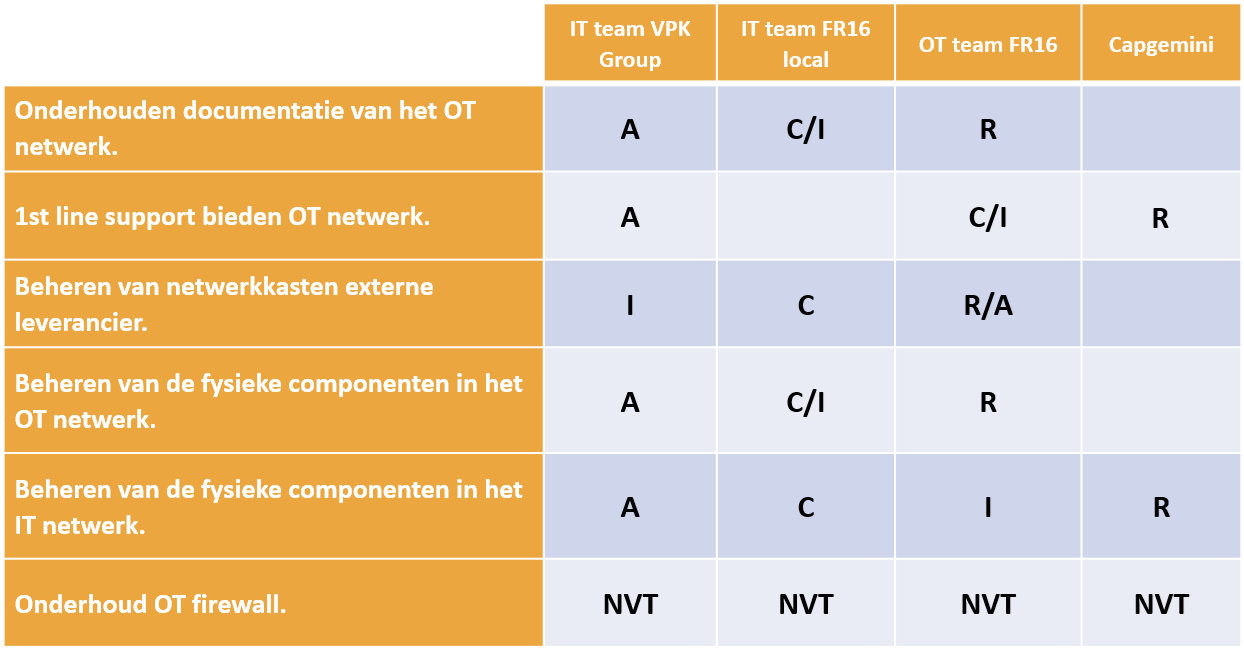
\includegraphics[width=0.9\textwidth]{fotos/Rasci_TO-BE.png}
    \caption[Foto Rasci TO-BE]{\label{fig:grail}Rasci tabel voor de toekomstige opstelling.}
\end{figure} 



\chapter{Configuratie van de firewall opstelling}

Op basis van de verzamelde info en de huidige problemen op de productiesite van Alizay, lijkt het logisch om te kiezen voor één soort firewall die goed past bij de bestaande infrastructuur en kennis binnen VPK. Een overstap naar een Palo Alto firewall heeft op dat vlak verschillende voordelen.

Met deze oplossing kan het beheer van alle firewalls binnen VPK op één plek gebeuren. Dat maakt het dagelijkse werk minder ingewikkeld. Ook gebruiken andere VPK-sites al Palo Alto, wat zorgt voor meer eenheid. Zo kan er beter gebruik gemaakt worden van bestaande kennis, werkwijzen en tools. Dit zorgt voor een veiligere en efficiëntere werking van zowel IT- als OT-netwerken. Tegelijk verkleint het de kans op fouten of verkeerde instellingen.

Doordat Palo Alto al op meerdere plaatsen binnen VPK gebruikt wordt, kan het netwerkteam sneller reageren bij problemen of aanpassingen doen zonder hulp van buitenaf nodig te hebben. Aangezien het huidige OT-netwerk vrij complex is, is het ook belangrijk dat de firewall goede ondersteuning biedt voor het opdelen van het netwerk, het opvolgen van verkeer en het beheren van wie toegang heeft tot wat.

Daarom lijkt het logisch om de Sophos firewall te verwijderen uit het netwerk, en enkel gebruik te maken van een Palo Alto firewall pair.

\newpage

\section{Beste High Availability settings voor de Palo Alto firewalls van FR16.}


High Availability (HA) is een functie die verschillende netwerk apparatuur vendors aanbieden, deze functie zorgt ervoor dat de downtime geminimaliseerd wordt door het gebruiken van meerdere entiteiten van dezelfde appartuur. Vaak zal er gebruik worden gemaakt van twee apparaten die dan op verschillende mogelijke manieren geconfigureerd kunnen worden. Twee populaire manieren om deze apparaten te configurenen zijn Active/Active of Active/Passive. De termen Active en Passive slaan hier op de staat van het apparaat. Active betekend dat dit apparaat weldegelijk bepaalde netwerk functies op zich zal nemen en dus actief zal meerwerken om bepaalde data te verwerken. Passive betekend dat het apparaat niet actief data zal verwerken, en zich dus in een soort van rust stand bevind.

\subsection{Active/Active firewall opstelling}
Bij een Active/Active opstelling verwerken beide apparaten actief data. In dit geval zullen beide firewalls gelijktijdig verkeer filteren op basis van vooraf gedefinieerde firewallregels. Hoewel dit in sommige situaties voordelen kan bieden, is deze opstelling in onze omgeving minder geschikt om meerdere redenen.


\begin{enumerate}
    \item \texttt{Active/Active firewall pairs zijn complex om te installeren en onderhouden: Sessie synchronisatie tussen de firewalls kan complex worden, zeker als er gebruik wordt gemaakt van dynamische IP’s binnen het netwerk. Omdat er is besloten in bovenstaande rasci matrix dat het beheer van de OT firewall een verantwoorddelijkheid is van het OT team lijkt het niet verstandig om gebruik te maken van een complexe firewall opstelling omdat de kennis over het beheer van dit soort opstellingen minder groot is bij het OT team.}
    
    \item \texttt{Kans op asymmetrische sessies: De kans is groter dat beide firewalls onafhankelijk data forwarden, waardoor inbound verkeer via een ander pad kan terugkeren dan outbound traffic. Dit kan leiden tot session mismatches, met als gevolg dat data mogelijk wordt gedropt.}  
    
    \item \texttt{Inconsistentie met andere sites: Alle andere VPK-sites met een Palo Alto firewall-pair gebruiken een Active/Passive-opstelling. Een Active/Active-configuratie binnen FR16 zou de uniformiteit van de netwerkarchitectuur verstoren}    
\end{enumerate}


Ook is binnen deze Active/Active opstelling de mogelijkheid om gebruik te maken van parallel processing. Dit zorgt er effectief voor dat throughput verdubbeld wordt. \autocite{Fulp2006} Voor onze use case is dit echter niet relevant. De hoeveelheid data die via de Sophos firewall wordt verstuurd, is zo laag dat één Palo Alto firewall ruim voldoende capaciteit heeft om deze load zonder merkbare vertraging te verwerken. Uit een uitgebreide analyse van het netwerkverkeer op de WAN poort van de Sophos firewall, uitgevoerd over meerdere weken en op verschillende tijdstippen, blijkt dat de maximale gemeten throughput slechts 10 KBps bedroeg.


De nieuwe Palo Alto firewall (PA-440) zou een maximale throughput van 2,6 Gbps hebben en ondersteunt 200.000 gelijktijdige sessies. \autocite{PaloAltoDS2025} Dit betekent dat de beschikbare capaciteit ruimschoots volstaat en dat een Active/Active configuratie geen toegevoegde waarde biedt voor deze specifieke productiesite.

\begin{figure}[H]
    \centering
    \fbox{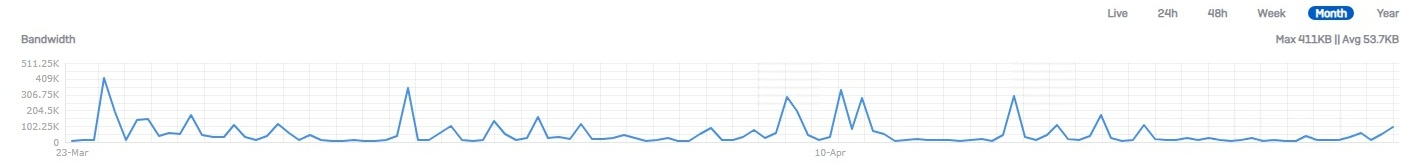
\includegraphics[scale=0.41]{fotos/SophosBandWidth.jpg}}
    \caption[PA High Availability settings]{\label{fig:grail}Totale bandbreedte die gebruikt wordt door de Sophos firewall op de productiesite van FR16}
\end{figure}




\subsection{Active/Passive firewall opstelling}

In een Active/Passive-opstelling is er slechts één firewall die gelijktijdig data verwerkt. Dit wordt mogelijk gemaakt door het configureren van HA-links. Deze links zijn cruciaal voor het waarborgen van redundantie, hoge prestaties en synchronisatie tussen firewalls in een HA-pair. Ze stellen de firewalls in staat om met elkaar te communiceren en statusinformatie te delen. Hierdoor kan de passieve firewall moeiteloos de taak van de actieve firewall overnemen bij een eventuele uitval. Zo zorgt de actieve firewall ervoor dat sessie-informatie wordt gedeeld met de passieve firewall, zodat deze altijd over de benodigde sessiegegevens beschikt in het geval van een failover. \autocite{PaloAltoHA2025} \autocite{PaloAltoHAb2025}

In hoofdstuk HOOFDSTUK NUMMER zal een HA verbinding tussen twee firewalls worden geconfigureerd op basis van de behoeften van VPK en de algemene best practices.

\begin{figure}[H]
    \centering
    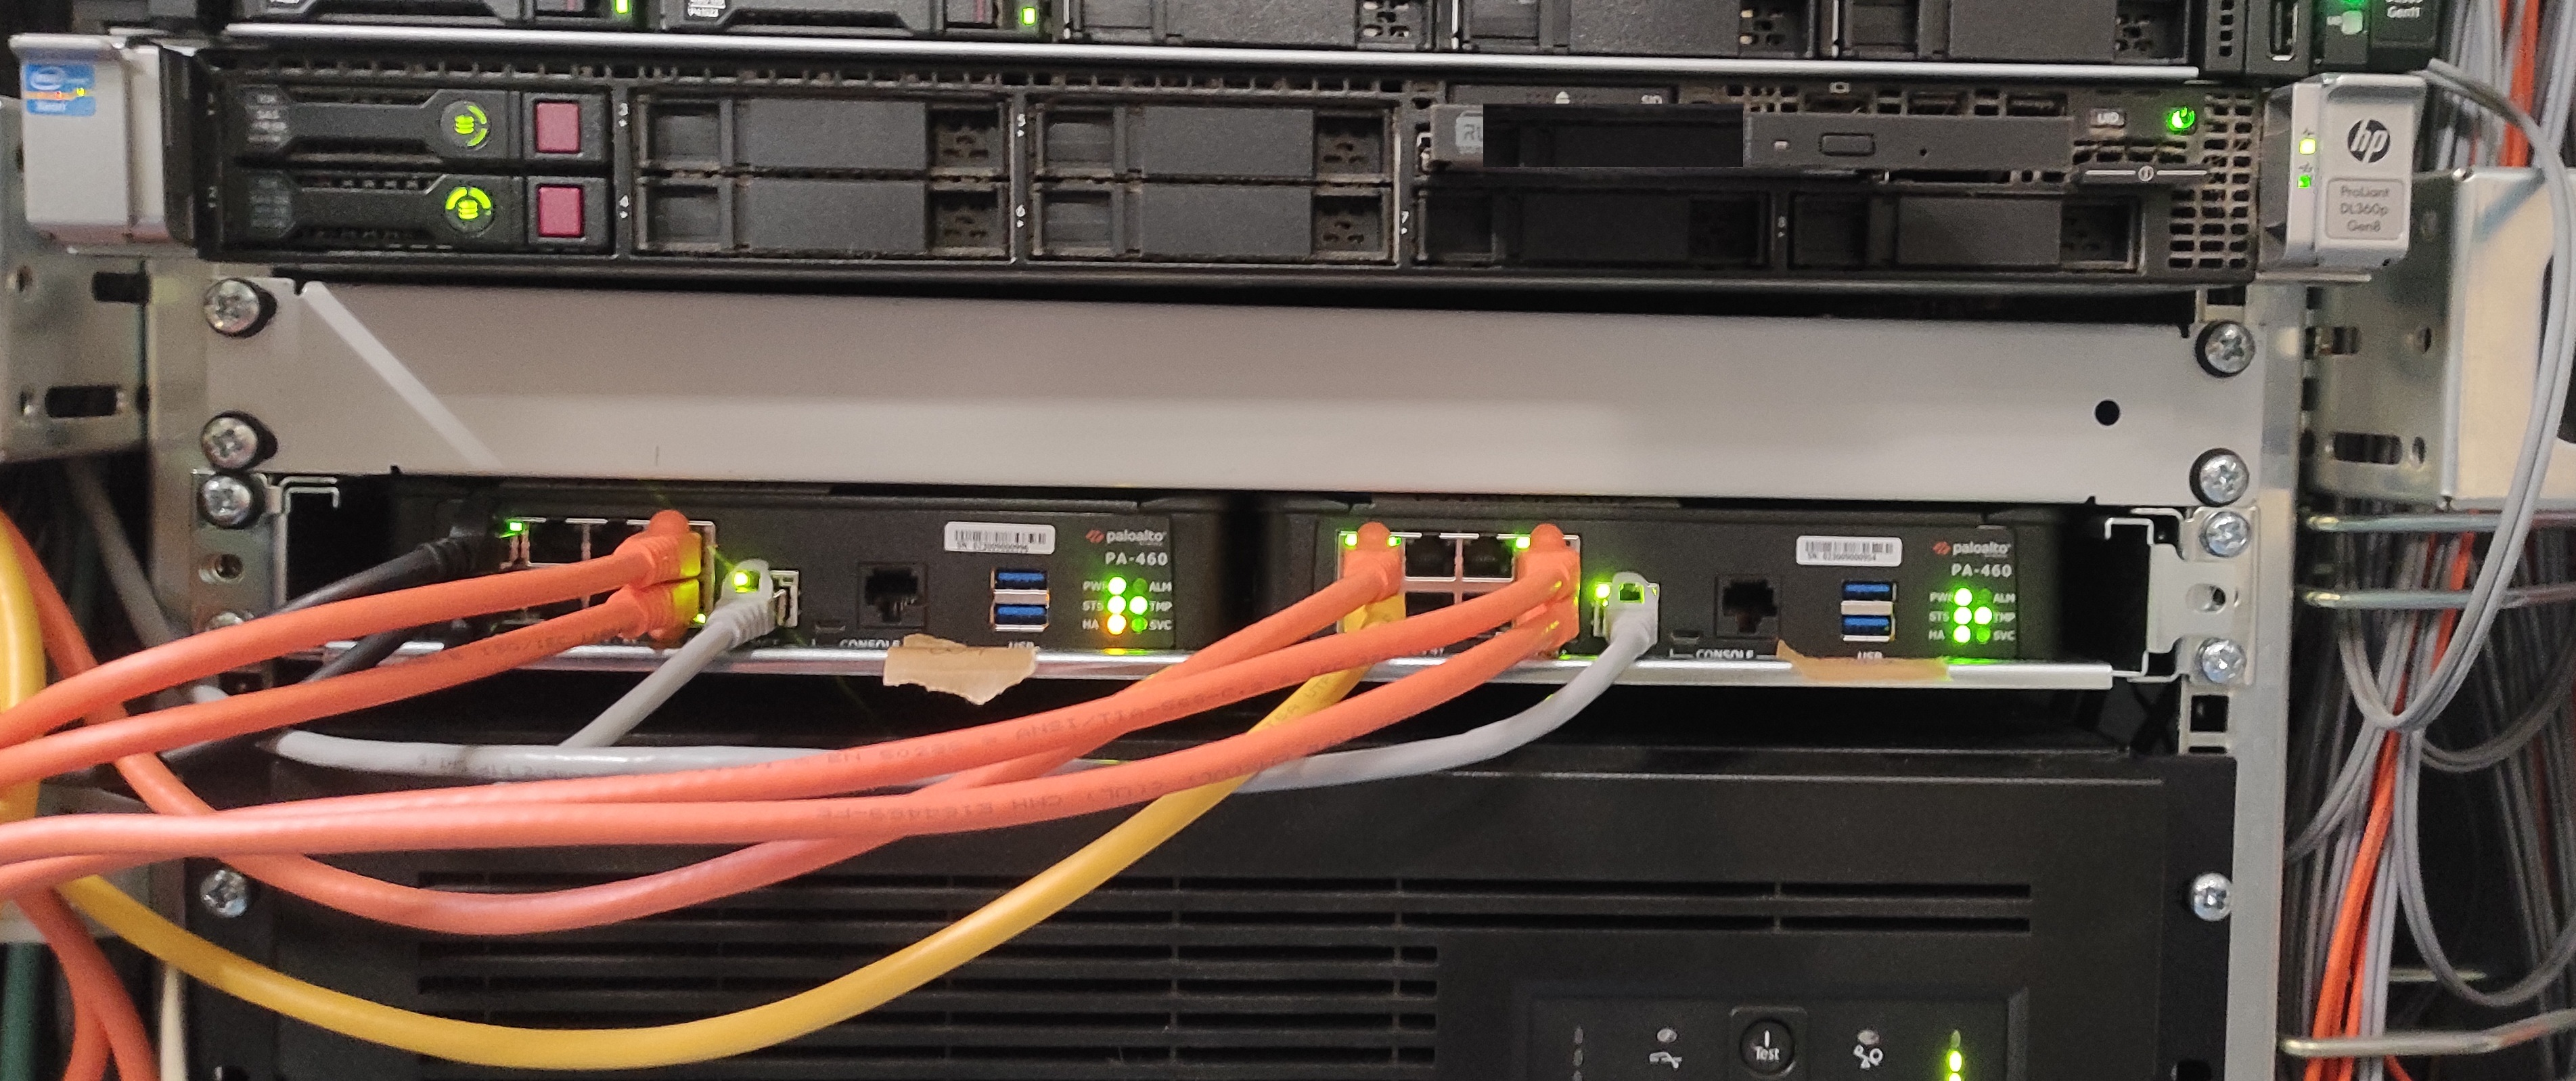
\includegraphics[width=0.8\textwidth]{fotos/PA_FirewallPairBE02.jpg}
    \caption[Palo Alto ACtive/Passive pair]{\label{fig:grail}Een Palo Alto Active/Passive firewall opstelling in één van de Belgische VPK sites}
\end{figure} 



\section{Beste High Availability settings voor de Sophos firewall van FR16}

Om gebruik te kunnen maken van de HA-functies van de Sophos firewall is het noodzakelijk om twee identieke firewalls aan te schaffen. Momenteel is er echter slechts één firewall aanwezig, waardoor VPK genoodzaakt zal zijn om een tweede Sophos firewall aan te kopen om HA te kunnen implementeren. Dit proces is echter niet eenvoudig, aangezien het onduidelijk is hoe de huidige Sophos firewall is geconfigureerd. Als de twee firewalls in het HA-paar verschillende instellingen hebben, kan dit in de toekomst mogelijk problemen veroorzaken. Daarom moet er een tweede identieke firewall worden aangeschaft, en is het essentieel om een onderzoek te doen naar de huidige configuratie van de Sophos firewall.



\section{Verzamelen en verwerken van Logs}

\subsection{Logs via Palo Alto}
De Palo Alto-firewalls die zich op andere locaties bevinden, verzamelen loggegevens van netwerkverkeer en systeemactiviteiten. Deze logs worden automatisch doorgestuurd naar een centrale server waarop Microsoft Sentinel draait. Microsoft Sentinel is een cloudgebaseerde SIEM-oplossing van Microsoft. SIEM staat voor Security Information and Event Management.
Volgens BRON verzamelt een SIEM systeem loggegevens uit verschillende bronnen, zoals firewalls, servers, toepassingen en andere netwerkapparaten. Die gegevens worden vervolgens geanalyseerd. Als er iets gebeurt dat afwijkt van het normale gedrag, kan Sentinel dit detecteren in realtime. Het systeem kan daarna automatisch meldingen sturen of zelfs actie ondernemen, zoals het blokkeren van een IP-adres of het starten van een onderzoek. Zo helpt Sentinel bij het vroegtijdig opsporen van cyberdreigingen en bij het verbeteren van de beveiliging van het netwerk.

FOTO SIEM Sentinel WIP (Ik heb zelf geen toegang tot deze portalen, er is een mail verstuurd naar de personen die hier wel toegang tot hebben.)


Naast Microsoft Sentinel worden de verzamelde loggegevens ook doorgestuurd naar de Zabbix monitoringserver. Zabbix is een open-source monitoringtool die gebruikt wordt om IT-infrastructuur te bewaken. Dit omvat onder andere fysieke servers, virtuele machines, netwerksystemen en cloudtoepassingen.
Zabbix verzamelt allerlei metrics zoals CPU-belasting, geheugengebruik, schijfruimte, netwerkactiviteit, enzovoort. Deze informatie wordt weergegeven in een overzichtelijk dashboard dat je via een webinterface kan bekijken. Zo kan er in één oogopslag gezien worden of er problemen zijn met een bepaald systeem of apparaat.
Zabbix maakt het ook mogelijk om alerts te versturen wanneer bepaalde drempels worden overschreden, bijvoorbeeld als de CPU belasting te hoog is of als een server niet meer reageert. Op die manier kunnen problemen snel worden gedetecteerd en opgelost, voordat ze ernstige gevolgen hebben.

FOTO Zabbix WIP (Ik heb zelf geen toegang tot deze portalen, er is een mail verstuurd naar de personen die hier wel toegang tot hebben.)


\subsection{Logs via Sophos}
Tot voor kort werden er op de Sophos-firewall geen loggegevens verzameld. Hierdoor was er weinig zicht op wat er zich precies afspeelde binnen het netwerkverkeer dat via deze firewall liep. Als onderdeel van mijn bachelorproef heb ik ervoor gezorgd dat de firewall nu wel logs verzamelt en dat deze op een correcte en veilige manier worden doorgestuurd naar de nodige servers die de data analyseren en verwerken.
De loggegevens worden via het syslog-protocol doorgestuurd naar twee verschillende servers: enerzijds de Zabbix monitoringserver en anderzijds de Microsoft Sentinel server. Deze syslog-berichten bevatten nuttige informatie, zoals de actuele firewallregels, de heartbeat van het systeem en verschillende systeemgebeurtenissen.
Omdat er op het FR16-netwerk tot nu toe nauwelijks of geen monitoring aanwezig was, is deze wijziging van groot belang. Dankzij deze aanpassing kunnen problemen sneller worden opgemerkt. In het geval van downtime of een mogelijke cyberdreiging kan er sneller worden ingegrepen, wat uiteindelijk helpt om schade of downtime te beperken.



\section{Configuratie van HA op een Palo Alto Firewall}

\textbf{Mode}
    \begin{itemize}[label=\textbullet]
        \item Zoals in hoofdstuk HOOFDSTUKNUMMER besproken zal er bij de configuratie van een Palo Alto firewallpair binnen een VPK site gebruik worden gemaakt van een Active/Passive opstelling. Hierbij zal er steeds slechts één firewall tegelijk actief zijn.
    \end{itemize}

\textbf{Enable Config Sync}
    \begin{itemize}[label=\textbullet]
        \item Configuration synchronization is een setting binnen Palo Alto HA firewall pairs. Waarbij een groot aantal settings automatisch worden gesyncroniseerd tussen devices. Om conflicten in configuraties te vermijden is het steeds aangeraden om configuraties steeds op de Active firewall uit te voeren en te wachten tot de Passive firewall gesynced is. Een aantal settings die niet worden gesynchroniseerd zijn: content updates, HA settings, mgmt interface settings, \ldots 
    \end{itemize}



\textbf{Passive Link state}
    \begin{itemize}[label=\textbullet]
        \item Deze settings zal bepalen in welke status alle data interfaces van een Passive firewall zullen worden geplaatst. Bij het gebruiken van de `shutdown` modus zullen alle data interfaces op de passive firewall in een `down` state worden geplaatst. Naast deze modus is er ook de `auto` modus. Bij deze modus zal alle data interfaces op `up` laten staan, maar dropped alle packets die over deze interfaces zouden passeren. Echter zou dit er voor kunnen zorgen dat switches nog steeds data packets zouden versturen over deze schijnbare `up` interfaces. Dit probleem samen met de algemene beste hardening cybersecurity practices om alle poorten die niet gebruikt worden op `down` te zetten zorgt ervoor dat VPK gebruik zal maken van de `shutdown` modus op beide firewalls.
    \end{itemize}



\textbf{Monitor fail hold time}
    \begin{itemize}[label=\textbullet]
        \item De ``monitor fail hold timer'' is een vooraf ingestelde timer om onnodige failover te voorkomen. Na dat één van de links down gaat zal het process geen nieuwe failover toestaan als het ziet dat er binnen de tijdslimiet van één minuut de interface terug `up` is. Mocht de link toch langer dan één minuut down zijn zal er toch een fialover gebeuren. Binnen iedere andere firewall op een VPK site wordt deze zelfde timer gebruikt. Daarom is er in het belang van uniformiteit gekozen om ook op deze site de timer in te stellen op één minuut.
    \end{itemize}



\textbf{Device Priority}
    \begin{itemize}[label=\textbullet]
        \item Deze settins zal bepalen welke prioriteit een bepaalde firewall heeft binnen een HA firewall pair. Een hogere waarde betekend direct ook een hogere prioriteit. Echter is dit enkel nuttig als men gebruik maakt van preemption. Maar aangezien preemption uit staat op deze firewalls zal deze priority waarde dus geen nut hebben.
    \end{itemize}



\textbf{Preemptive}
    \begin{itemize}[label=\textbullet]
        \item Deze setting zal er voor zorgen dat de firewall met een hogere prioriteit in staat is om terug Active te worden nadat er een failover is gebeurd. Echter heeft VPK gekozen om deze setting niet in te schakelen bij alle firewalls op alle VPK sites.
    \end{itemize}



\textbf{Hearbeat backup}
    \begin{itemize}[label=\textbullet]
        \item Deze optie zorgt ervoor dat er een backup is om de hearbeat berichten van de apparaten op te sturen via de management interfaces van de firewall. Deze berichter zullen standaard over de HA1 en HA2 link worden verstuurd. Aangezien er twee rechtstreekse linken zijn tussen de twee firewalls in het HA pair is het dus niet meer nodig om deze optie aan te zetten.
    \end{itemize}


\begin{figure}[H]
    \centering
    \fbox{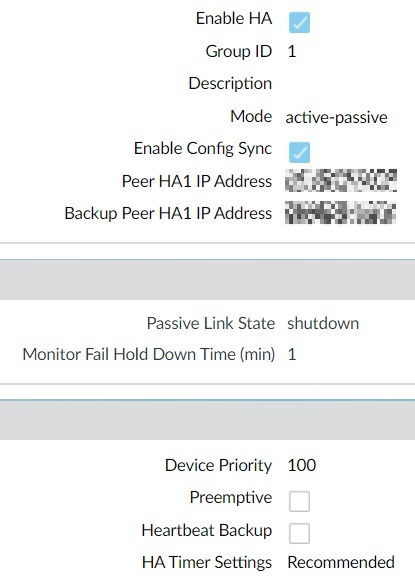
\includegraphics[scale=0.666]{fotos/PA_HASettings.jpg}}
    \caption[PA High Availability settings]{\label{fig:grail}GUI interface om de settings om de configuratie van High Availability op een PA firewall aan te passen.}
\end{figure}


\section{Netwerksegmentatie aan de hand van VLAN’s}

Netwerksegmentatie met VLAN’s (Virtual Local Area Networks) is nog steeds een erg goede manier om verschillende delen van een netwerk virtueel van elkaar te scheiden. Daarom lijkt het een slim idee om deze techniek ook toe te passen op het VPK-netwerk.

Concreet kan ervoor gekozen worden om de apparaten die binnen het IT/OT netwerk actief zijn onder te verdelen in verschillende groepen. Zo worden deze groepen van elkaar afgescheiden en is communicatie tussen hen standaard niet meer mogelijk. Uiteraard kunnen we nog steeds toestaan dat bepaalde groepen met elkaar praten via firewallregels op de Palo Alto firewall.

Het belangrijkste doel hiervan is simpel: als een aanvaller erin slaagt om toegang te krijgen tot één apparaat, dan krijgt hij niet meteen toegang tot het volledige netwerk, maar blijft hij beperkt tot het VLAN waarin dat toestel zich bevindt.

Om het allemaal overzichtelijk te houden, is het ook aangeraden om de VLAN’s te koppelen aan specifieke IP-ranges. Zo is het makkelijker om snel te zien in welk VLAN een bepaald toestel zit.

\subsection*{Voorbeeld VLAN-indeling}

\begin{table}[h!]
    \centering
    \begin{tabular}{|l|l|c|l|l|c|}
        \hline
        \textbf{DHCP} & \textbf{Usable range} & \textbf{VLAN} & \textbf{Name} & \textbf{Gateway} & \textbf{Mask} \\
        \hline
        10.x.2.0 & 10.x.2.1 -- 10.x.2.240 & 2 & AP mgmt & 10.x.2.254 & /24 \\
        10.x.4.0 & 10.x.4.1 -- 10.x.4.240 & 4 & Switch mgmt & 10.x.4.254 & /24 \\
        10.x.8.0 & 10.x.8.1 -- 10.x.8.240 & 8 & Server & 10.x.8.254 & /24 \\
        10.x.9.0 & 10.x.9.1 -- 10.x.9.240 & 9 & RF\_Corporate & 10.x.9.254 & /24 \\
        \hline
    \end{tabular}
    \caption{VLAN's en bijhorende IP-ranges}
\end{table}

Uit het bovenstaande voorbeeld kan je afleiden dat er gekozen is om binnen VPK VLAN 8 te gebruiken voor alle servers binnen het netwerk. Zo weten we meteen dat een toestel met een IP-adres in de vorm van x.x.8.x een server is. Deze manier van werken brengt verschillende voordelen met zich mee:

\begin{itemize}
    \item \textbf{Overzichtelijkheid:} Door vaste IP-ranges per VLAN te gebruiken, is het snel duidelijk tot welke categorie een toestel behoort. Dit maakt het beheer en de troubleshooting veel eenvoudiger.
    \item \textbf{Beter beveiligd:} Apparaten die tot dezelfde functie horen (zoals servers) zitten samen in één VLAN. Dit beperkt de schade als er iets misloopt.
    \item \textbf{Efficiëntere netwerkconfiguratie:} Firewalls en andere beveiligingsregels kunnen veel gerichter ingesteld worden.
    \item \textbf{Makkelijker uitbreidbaar:} Je weet meteen in welke IP-range nieuwe toestellen moeten komen.
    \item \textbf{Snellere probleemoplossing:} Het IP-adres geeft snel inzicht in het type toestel en het netwerksegment.
    \item \textbf{Uniformiteit over verschillende sites:} Eén consistente VLAN-structuur vergemakkelijkt het beheer over meerdere locaties.
\end{itemize}

In het netwerk kan er ook voor gekozen worden om elke externe leverancier in een aparte VLAN onder te brengen. Bijvoorbeeld: Minda, Ducker, Bobst en Gopfert hebben elk hun eigen VLAN en aparte IP-range. Dit biedt heel wat voordelen:

\begin{itemize}
    \item \textbf{Verhoogde veiligheid:} Problemen blijven beperkt tot de VLAN van de leverancier.
    \item \textbf{Gerichte toegangscontrole:} Per VLAN kan je precies bepalen welke toegang een leverancier krijgt.
    \item \textbf{Compliance:} Helpt bij het voldoen aan interne en externe auditvereisten.
\end{itemize}

\section{Verschillende fases bij het deployen van firewall rules}

Bij de implementatie van de nieuwe firewalls wordt er gekozen om de firewallregels gefaseerd uit te rollen. Dit betekent dat niet alle regels in één keer actief worden, maar dat het netwerk stap voor stap verder wordt afgeschermd. Door steeds specifiekere regels in te voeren.

\subsection*{Voordelen van gefaseerde implementatie}

\begin{itemize}
    \item \textbf{Minder risico:} Fouten worden sneller opgemerkt en bijgestuurd.
    \item \textbf{Eenvoudigere probleemoplossing:} Door de gefaseerde aanpak kan men sneller de oorzaak van problemen vinden.
    \item \textbf{Beperkte OT documentatie:} Onverwachte sessies kunnen zonder onmiddellijke blokkering worden geanalyseerd.
    \item \textbf{Minimale impact op bedrijfsprocessen:} Kritieke toepassingen blijven beschikbaar tot in de laatste fase.
\end{itemize}





